\section{Introduction}

The Vera C. Rubin Observatory\cite{2019ApJ...873..111I} will go in to operations in 2025.
During commissioning we have already seen our infrastructure as code based cyber system working well.
In this paper we will describe the generic underlying hardware, deployments on that hardware of both bare metal and containerized applications, transmission of data to SLAC and our NIST\cite{NIST.SP.800-171} compliant security approach.

The Rubin summit may be viewed in terms os standard Cyber Infrastructure Layers.
The layers are graphically depicted in \figref{fig:ci-rubin}i which is a revised version of the diagram presented in \cite{2019arXiv190713060O}.
Each layer is covered in a section below as follows:

\begin{enumerate}
\item The physical layer covered in \secref{sec:physical}
\item The network layer covered in \secref{sec:networking}
\item The computing layer covered in \secref{sec:computing}
\item The application layer covered in \secref{sec:application}
\end{enumerate}


\begin{figure}
\begin{centering}
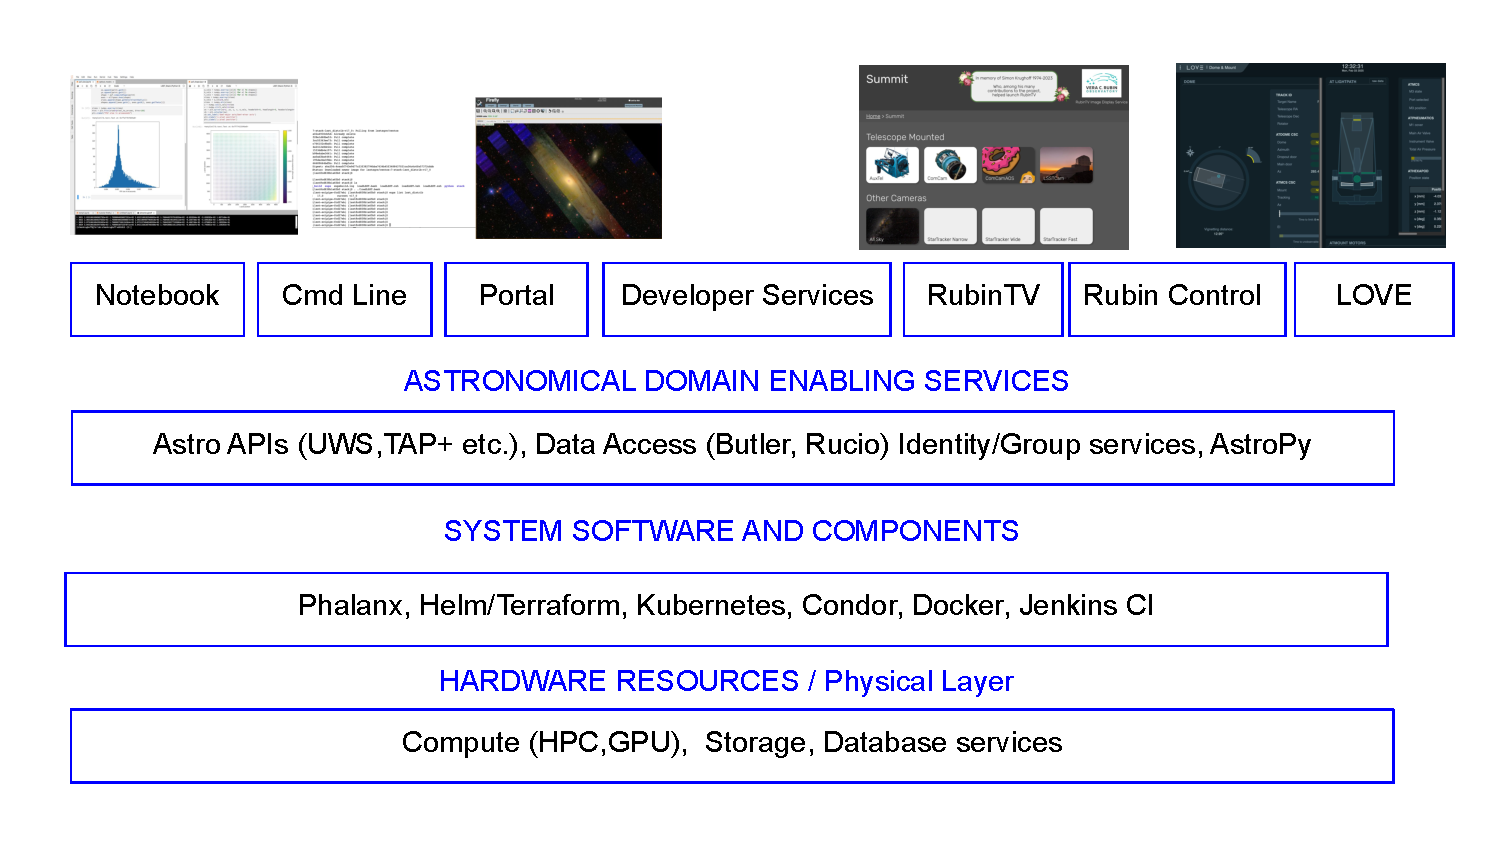
\includegraphics[width=0.9\textwidth]{images/CI-Rubin}
	\caption{Rubin Cyber infrastructure layers
\label{fig:ci-rubin}}
\end{centering}
\end{figure}


\section{Physical Layer} \label{sec:physical}

\subsection{Design}
Scalability, Open design

\subsection{Legos}
Blocks

\section{Networking Layer} \label{sec:networking}

\subsection{Reliability}

\subsection{Scalability}

\section{Computing Layer} \label{sec:computing}

\subsection{Automatizing}
IaC, GitOps, CI/CD

\subsection{Monitoring}
Health, Logs, Dashboards, Alerts

\section{Application Layer} \label{sec:application}

\subsection{Deployments}
Test Stands, Canary, Blue/Green

\subsection{Security}
Detections, Identities, Monitoring

\section{Incidents Management}
Alerts, Escalation,

\section{Documentation}
Technotes, Runbooks
